\section{System Design}\label{s:arch}
\sys combines query distribution predictions, a push-based streaming model, and progressive results into an efficient and low-latency interactive visualization architecture.  In this section, we describe the architectural design and the key technical challenges.

\begin{figure}[tb]
	\centering
	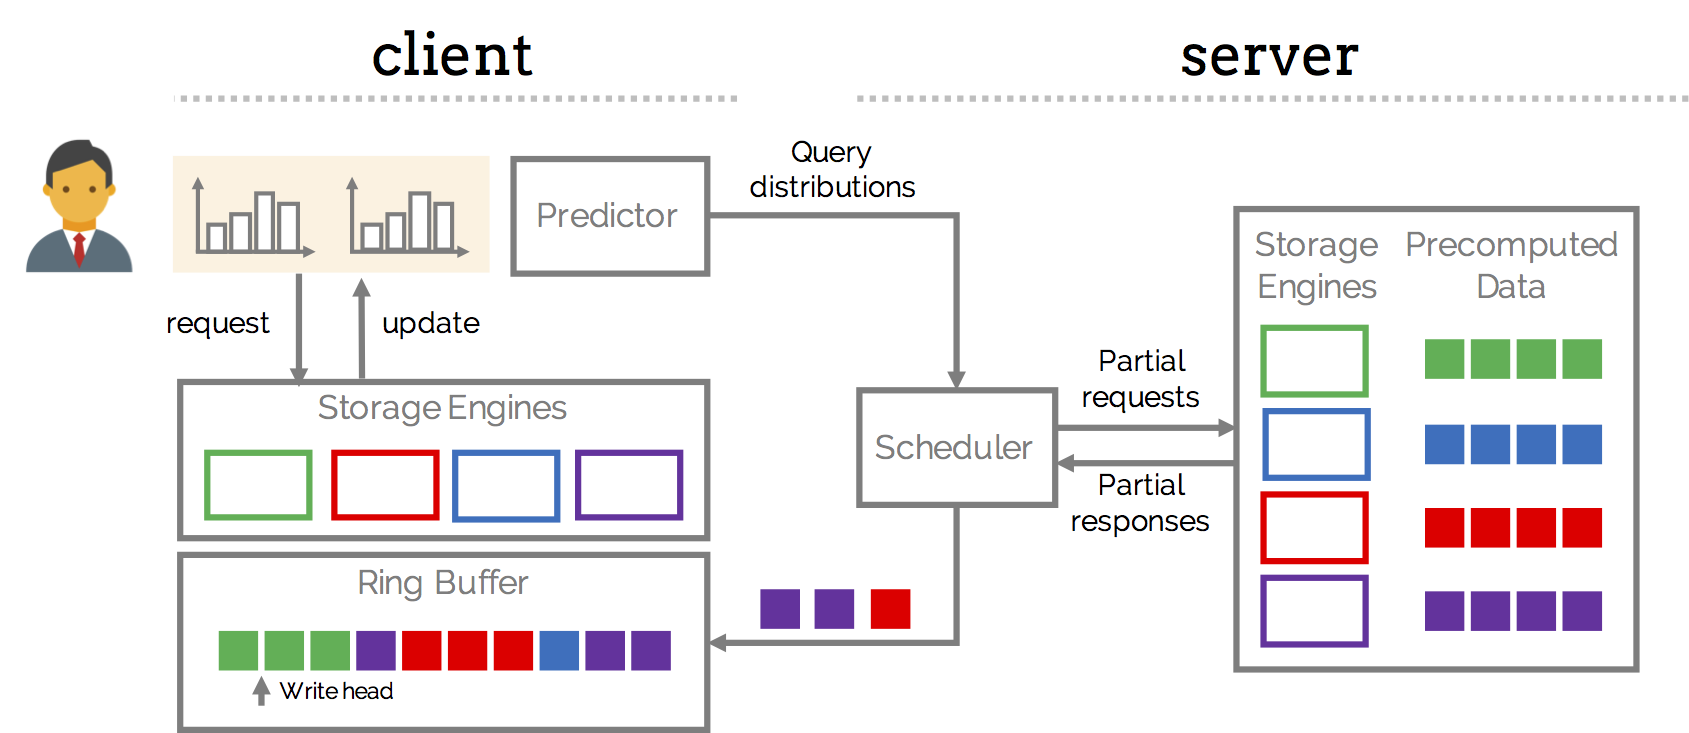
\includegraphics[width=\columnwidth]{figures/arch}
 	\caption{\sys Architecture}
  \label{fig:arch}
\end{figure}

\subsection{Architecture}

\sys is a streaming system designed for low-latency, data intensive interactive visualization systems.  It  consists of a thin client, such as a modern web browser, that has a limited cache size, and a more powerful backend server that answers client queries and pre-computes physical data structures during an offline optimization phase.  

In order to improve perceived user interaction latency, \sys decouples client requests from server responses---the client periodically sends predictions at a rate that does not interfere with user interactions and rendering, and the server continuously sends a stream of results to the client. 

Figure~\ref{fig:arch} presents the overall system architecture.
The user interacts with an interactive visualization that we model as queries over an underlying database~\cite{wucombining,EugeneWuVision2014}.  The client keeps a cache of data in the {\it Ring Buffer}; if the request can be answered by the cache, then the visualization immediately updates.  Otherwise, the client must send a request to the server similar to traditional request-response systems.

The {\it Predictor} is a separate thread that monitors the user's mouse movements ad interactions to make predictions about the user's future interactions.  These predictions are modeled as distributions over a query space, similar to the Query Intent model by Nandi et al.~\cite{gesturequery}, and sent to the server {\it Scheduler}.

 Although any existing interaction or query predictor~\cite{} can be plugged into this component, we have found that their prediction accuracy degrades significantly (e.g., \ewu{XXX accuracy}) in even linked-brushing bar chart visualizations (Figure~\ref{fig:barchart}).  The primary reason is that the user can interact with any of the \ewu{100} bars, which presents a sparse state space that is challenging for existing predictors.


The {\it Scheduler} monitors the changes in the query distributions, allocates portions of the network connection to each query, retreives partial results and determines the order they are sent back to the client.  The scheduler simply schedules and routes queries, which are executed by the {\it Storage Engines}.  Each storage engine is responsible for implementing two functions.     \texttt{costEstimate(query):Int} returns a rough cost estimate to execute the query, or $-1$ if it is not able to; this allows a storage engine to restrict the set of queries it must answer, and thereby allow hyper-specialized storage engines.  \texttt{getBytes(query, nBytes, [offset]):ByteBuffer} executes the query and returns the most informative \texttt{nBytes} to approximate those results; the optional third argument specifies that the client already recieved the first \texttt{offset} bytes.

For instance, a naive storage engine may pre-compute results for a parameterized query.  Given \texttt{SELECT a, sum(b) FROM T WHERE c = ? GROUP BY a}, the engine may execute the query for all assignments of \texttt{c}, and perform wavelet compression on each result~\cite{malvar1999fast}.  Since the results are precomputed, the \texttt{costEstimate} is simply a constant lookup cost if the query matches the template, or $-1$.  Finally, because the results are progressively encoded, the engine returns the first \texttt{nBytes} of the precomputed results.  

Each server-side storage engine has a client-side counterpart that is responsible for decoding the byte streams and returning query results in the form of relations.  This design gives each storage engine flexibility in how it encodes the data.  For instance, a sampling-based storage engine may simply send samples to the client, which performs aggregation and approximation over all samples in the ring buffer.  Similarly, a datacube-based storage engine may send relevant portions or resolutions of the datacube to the client.

Ultimately, the Scheduler sends the bytes it retrieves from the storage engines to the client's ring buffer.  The {\it Ring Buffer} is akin to the buffer manager in classic database systems.  It is a preallocated block of memory; however in contrast to traditional buffer managers, data sent from the server is written sequentially to the buffer and simply overwrites existing content. \ewu{Explain the rationale for this.} Every time the ring buffer detects a usable block of bytes, it sends a view of the block to its appropriate client-side storage engine to decode and use to answer client queries.  Similarly, when a block is overwritten, it sends a \texttt{deallocate} request to the appropriate storage engine.

\subsection{Design Rationale}

Visualization systems typically restrict the query space to a finite set of pre-defined query structures.    In our case, we simplify and assume a set of query templates have been pre-registered to the system.  This is common in data intensive graphics and visualization systems~\cite{wireviz}


This design is based on a confluence of powerful browser javascript engines and unbiquitous networking.  The advent of powerful browser technologies such as vectorized execution and asm.js-based Ahead-of-time compilation has led to the possibility of browser-based query execution engines whose performance is competitive with state-of-the-art in-memory column store databases such as MonetDB~\cite{gebaly2016afterburner}.

\ewu{Maybe cut?  Although the physical implementation is client server, the logical analysis considers the data visualization as a logical database view~\cite{EugeneWuVision2014,wucombining}}


\subsection{Technical Challenges}

Challenges:   How to represent and generate distributions?
What to return?  Scheduling problem -- adopt existing scheduling work.
Progressive encoding -- try obvious options.  see if they work.


